\chapter{はじめに}
\label{introduction}

\section{研究背景}
\label{subject}
``Embodiment''という言葉が、心理学やロボティクス、バーチャルリアリティ(VR)、ヒューマンインターフェースデザインなど、さまざまな分野で注目されている。Botvinick \& Cohenによるラバーハンド錯覚\cite{BotvinickCohen1998}の報告は、私たちが自分の身体として認知する対象は生まれ持った肉体に限らないことを示した。それを皮切りに、「私たちはどこまでを自分の身体として認識しうるか?」、すなわち「何を``身体化''できるのか?」について、その可能性と限界を探る研究が次々と発表されている。また、インターフェース研究者の渡邊は「まさに自分自身の身体である」という感覚を指すGallagher\cite{Gallagher2000}の``sense of ownership''を「自己帰属感」と訳し\cite{Watanabe2013}、インターフェースにおける直感操作を実現する重要な指針として、「身体化」の議論との橋渡しをした。Embodimentの訳は「身体化、一体化、身体性」など文脈によって異なるが、これらについては「私たちの身体に帰属する他者」に注目しているという点で、「身体化」と訳すことが適当だと思われる。こうした「``身体化''としてのembodiment」は、人間の可能性の拡張や、直感的で便利なインターフェースを実現するためのデザインへの応用へと広がっている。

% インターフェース研究者の渡邊は、インターフェース設計における理想形を「透明化」であると説明する\cite{Watanabe2017}。すなわち、どんなに複雑で高度な道具であっても、原始的な道具のように原因と結果の関係が直接的であり、道具そのものに対して意識することなくそれを使用できることこそが理想とした。

% そして渡邊は、その理想を実現するための重要な指針が「自己帰属感(sense of ownership)」であると提言する。自己帰属感とは、「あたかもその装置が身体の延長であるかのように感じられる」感覚を指す。

% 人々を取り巻くものが機械や情報処理によって高度化する中、人々と機械との接点を設計することが重要となった。
% ここで、人々と機械との最適な関係を「より使いやすく有用に」 \footnote{国際標準化機構(ISO)による「人間中心設計」の導入部\cite{hcd}より}することとし、それを具現化してきたのがエルゴノミクス、人間中心設計といった設計論である。

% 道具の使用における行為と結果の関係から捉えたとき、「使いやすさ」とは、原始的な道具のように直接的であり、道具そのもに対する意識がなくなっていく「透明化」を指す。

% 渡邊は、その理想を実現する指針として「自己帰属感」という概念を導入し、例えばマウスカーソルやスマートフォンのような「操作時の指とグラフィックの追従性が高い」インターフェースは自身の一部や延長として感じられる、「透明」なインターフェースであると説明する。

% こうした設計論は、確かに複雑で高度な道具の力を借りて人間の活動の可能性を拡げることに貢献してきた。
しかし、自己と他者との関係には、「他者に帰属する私たち」という関係も存在するのではないだろうか。例えばそれは、ピアノと人との間にある。ピアノを初めて弾くとき、奏者は手の大きさによる制約から、左右別々に指を動かすだけでも困難さを経験する。しかし、試行錯誤を経て、ピアノの制約と自身の身体能力との間で折り合いをつけていくことで、ようやく楽器を通して表現ができるようになる。ミュージシャンのスキャットマン・ジョン(ジョン・ポール・ラーキン)は、「吃音症」という発話障害を抱え、「自身の身体」という切っても切り離せない存在をコントロールできない中、むしろその症状を逆手に取るように「テクノスキャット」という独自の歌唱法を開拓した。このようにして他者と調和していくことは、これまでの議論に潜在していても、注目されてこなかったembodimentの側面と言えるのではないか。

こうした関係について考えるにあたっては、embodimentを「自己」と「他者」の関係に対して中立的な``一体化''と訳すことが適当だと考える。そして、「自己」と「他者」のあいだで折り合いをつけていくようなこの``一体化''は、インタラクションの中でその人自らの学習ややり方の創造プロセスがあって初めて芽生えることから唯一性があり、また困難を乗り越えていく過程に人間にとっての根源的な喜びがあると考える。

そこで本研究では、「自己」と「他者」の双方向的な折り合いによる一体感である「人馬一体」という関係に注目した。「人馬一体」化のプロセスは、人と馬だけに限らず例えば楽器やバイクなどにもみられる、それに合わせて自分の振る舞いを変化させることで、唯一性のある関係を育むことであると考える。

これを具現化するような関係性が芽生える体験は、いかにして設計できるのか。本研究では、手指の変換表現を通して人馬一体のような「一体感」のデザインを目指す。

% \section{リサーチクエスチョン}
% \label{research_question}
% 前節では、研究背景に触れ、本研究が「人馬一体」と言われるような、相互の折り合いをつけながら生まれる親密さについて探索するものであると説明した。ここでは、探索の上での中心的な問いについて明記する。

% \begin{quote}
% \textbf{対象からの影響も受けつつ、相互の折り合いをつけながら生まれる一体感はどのように生まれるのか。そして、それはいかに設計できるのか。}(最後に回収)
% \end{quote}


\section{手指の変換表現から「人馬一体」感を探求する動機}
\label{prototyping_concept_making}
本研究が注目する「人馬一体感」は、自分と自分でないもの(道具、機械、他の人間、あるいは文字通り、馬のような異種の生物など)の間に生起するものである。そのため具体的に人と何の「関係」を分析し、デザインするかについては選択の余地がある。本研究では、人と「変換された手指」との関係から取り組んだ。そのきっかけとなったのは、もとは別の目的で制作していた習作「Digitize」である。この習作を展示した際、体験者と作品との関係が、これまで経験したことのない特異なものであったことに興味を抱いた。この作品が、本研究の動機となった。これより、その習作について説明し、それがどのような関係であったのかについて述べる。

習作「Digitize」とは、手指の動きを別の形へとマッピングさせた3つの変換表現から構成された作品である。静止画について構想を膨らませる際、私たちは「紙とペン」を通して直接イメージをスケッチできる。動きについてもそれに相当するほど、直感的かつ、高い表現力でスケッチができるツールを作ろうとした。そこで、動きに対して高い表現力を有する手指を使って、「動きをスケッチする」ツールを案じていた。しかし手指の動きをそのまま表示するのでは、手指を使うことの意義が薄い。手指は人間の身体の中でも高い表現力をもつ器官である。もし「手ではない形」を通してでも、様々な形や動きを自由に作れるのなら、人間の身体構造による制約を超えた「動きのスケッチ」ができ、手指を使うことの意義があるのではないかと構想した。そうして、手指の動きをトラッキングするが、画面上では別の形へマッピングされて動くインターフェースについて、プロトタイピングを行った。

この習作を起点に、動きのスケッチツールとしての構想を深める目的のもと、2022年7月に岐阜県大垣市で開催されたイベント「IAMAS OPEN HOUSE 2022」にて展示した \footnote{\url{https://k1105.github.io/eee_openhouse_2022/}}。この時点では、動きを記録する機能はなく、あくまで手指とは異なる形状が手の動きに伴って動くのを確認するだけのものであった。

\begin{figure}[H]
  \centering
  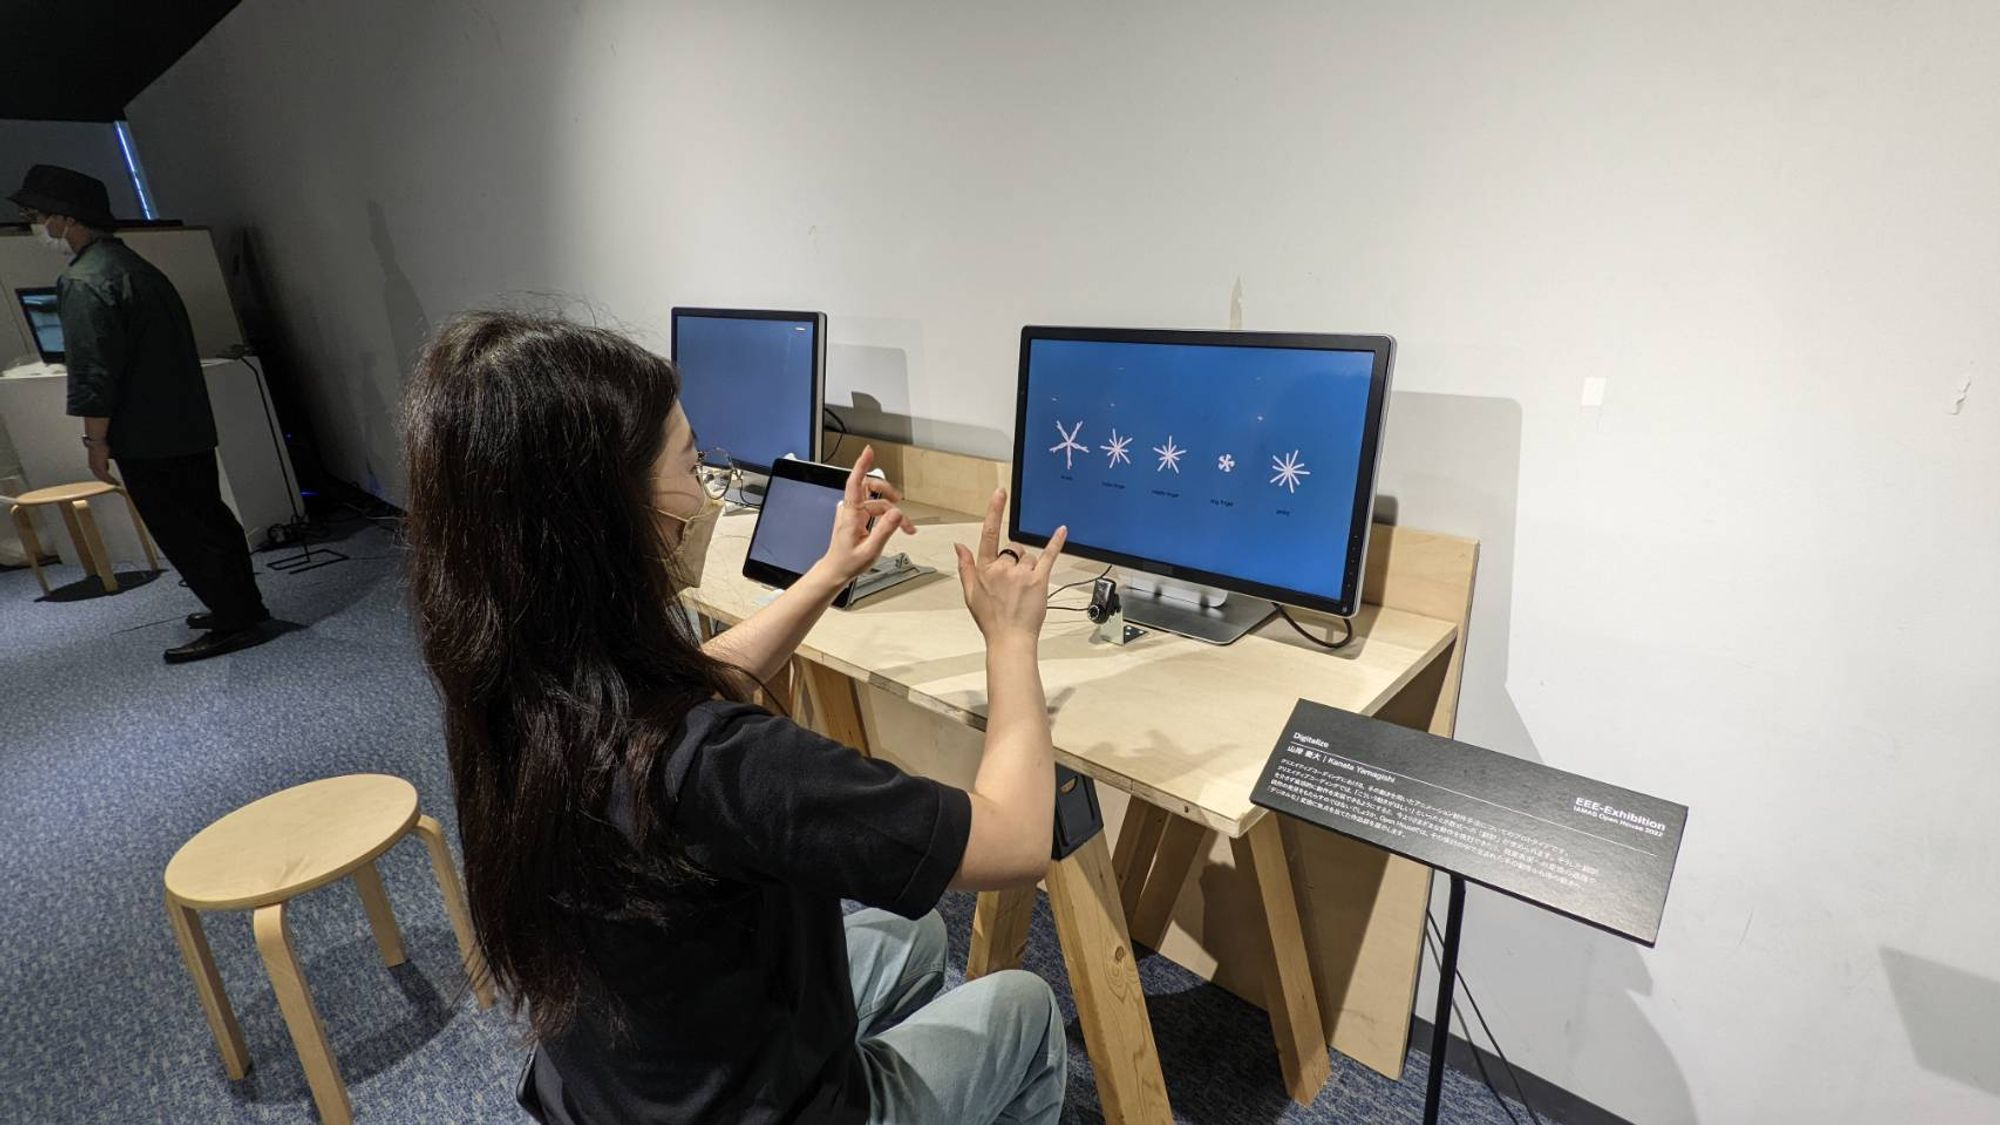
\includegraphics[width=15cm]{img/openhouse2022.jpeg}
  \caption{IAMAS OPEN HOUSE 2022での展示の様子(2022年)}
  \label{fig:exhibit_2022}
\end{figure}

\begin{figure}[H]
  \centering
  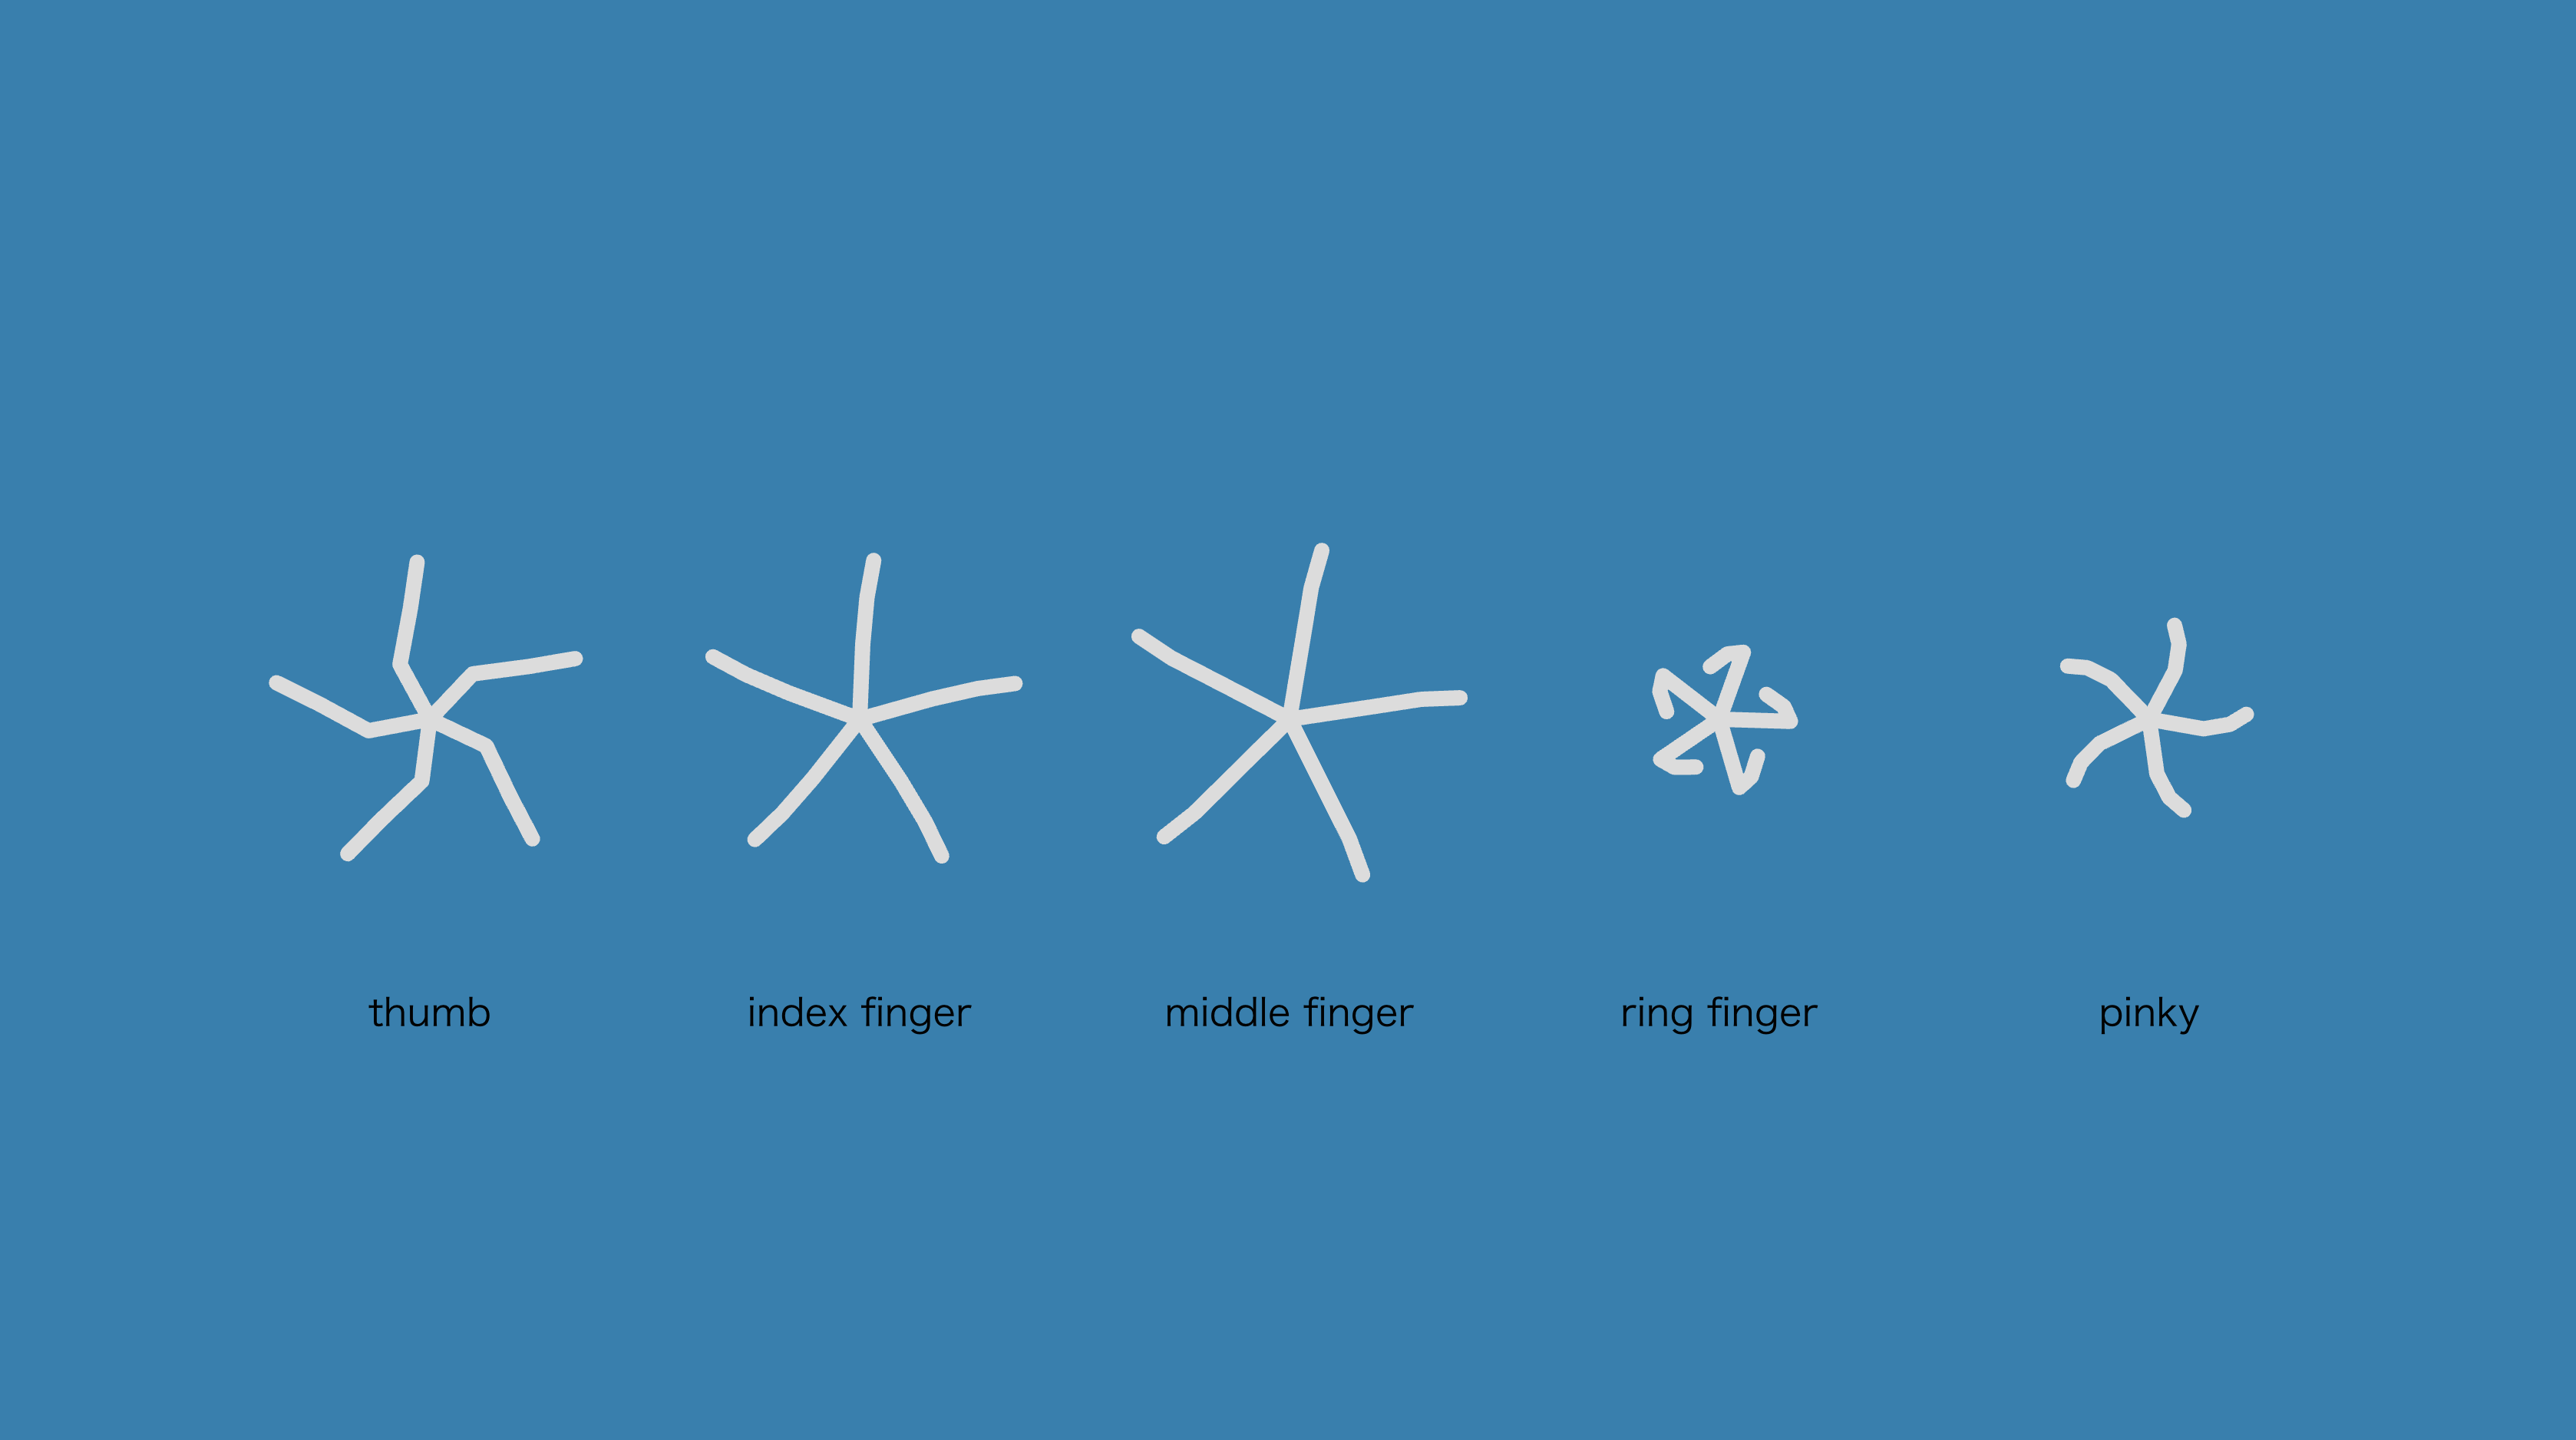
\includegraphics[width=15cm]{img/openhouse2022_interface.png}
  \caption{Digitizeのインターフェース(2022年)}
  \label{fig:exhibit_2022_interface}
\end{figure}

しかし展示を行うと、想定していなかった体験の様子が見られた。それは、この変換に対していくつかの異なる解釈が生まれたことである。例えば図\ref{fig:exhibit_2022_kunoji}に示す「くの字」が並んだパターンは、その一つ一つが、カメラから取得された指先から付け根のy軸方向の距離に応じて屈曲する。それは作者が、画面の前でも同じように手の指を屈曲させて動かすことを期待してのことだった。しかし実際には、まったく違う方法でそれを操る体験者が現れた。例えば、図\ref{fig:movement_0}に示すように指ではなく、手首を回転させることで操作する体験者がいた。また、カメラに対して手を近づけたり、遠ざけたりすることで屈曲させる体験者がいた。この方法でも動作するのは、カメラに対する手指の距離が変わることで、認識される手の大きさ自体が変化するためである。さらに図\ref{fig:movement_1}のように、高速な動きに対するトラッキングの追従精度から生じるある意味「バグ」の挙動を用いて動かす体験者が現れた。

\begin{figure}[H]
  \centering
  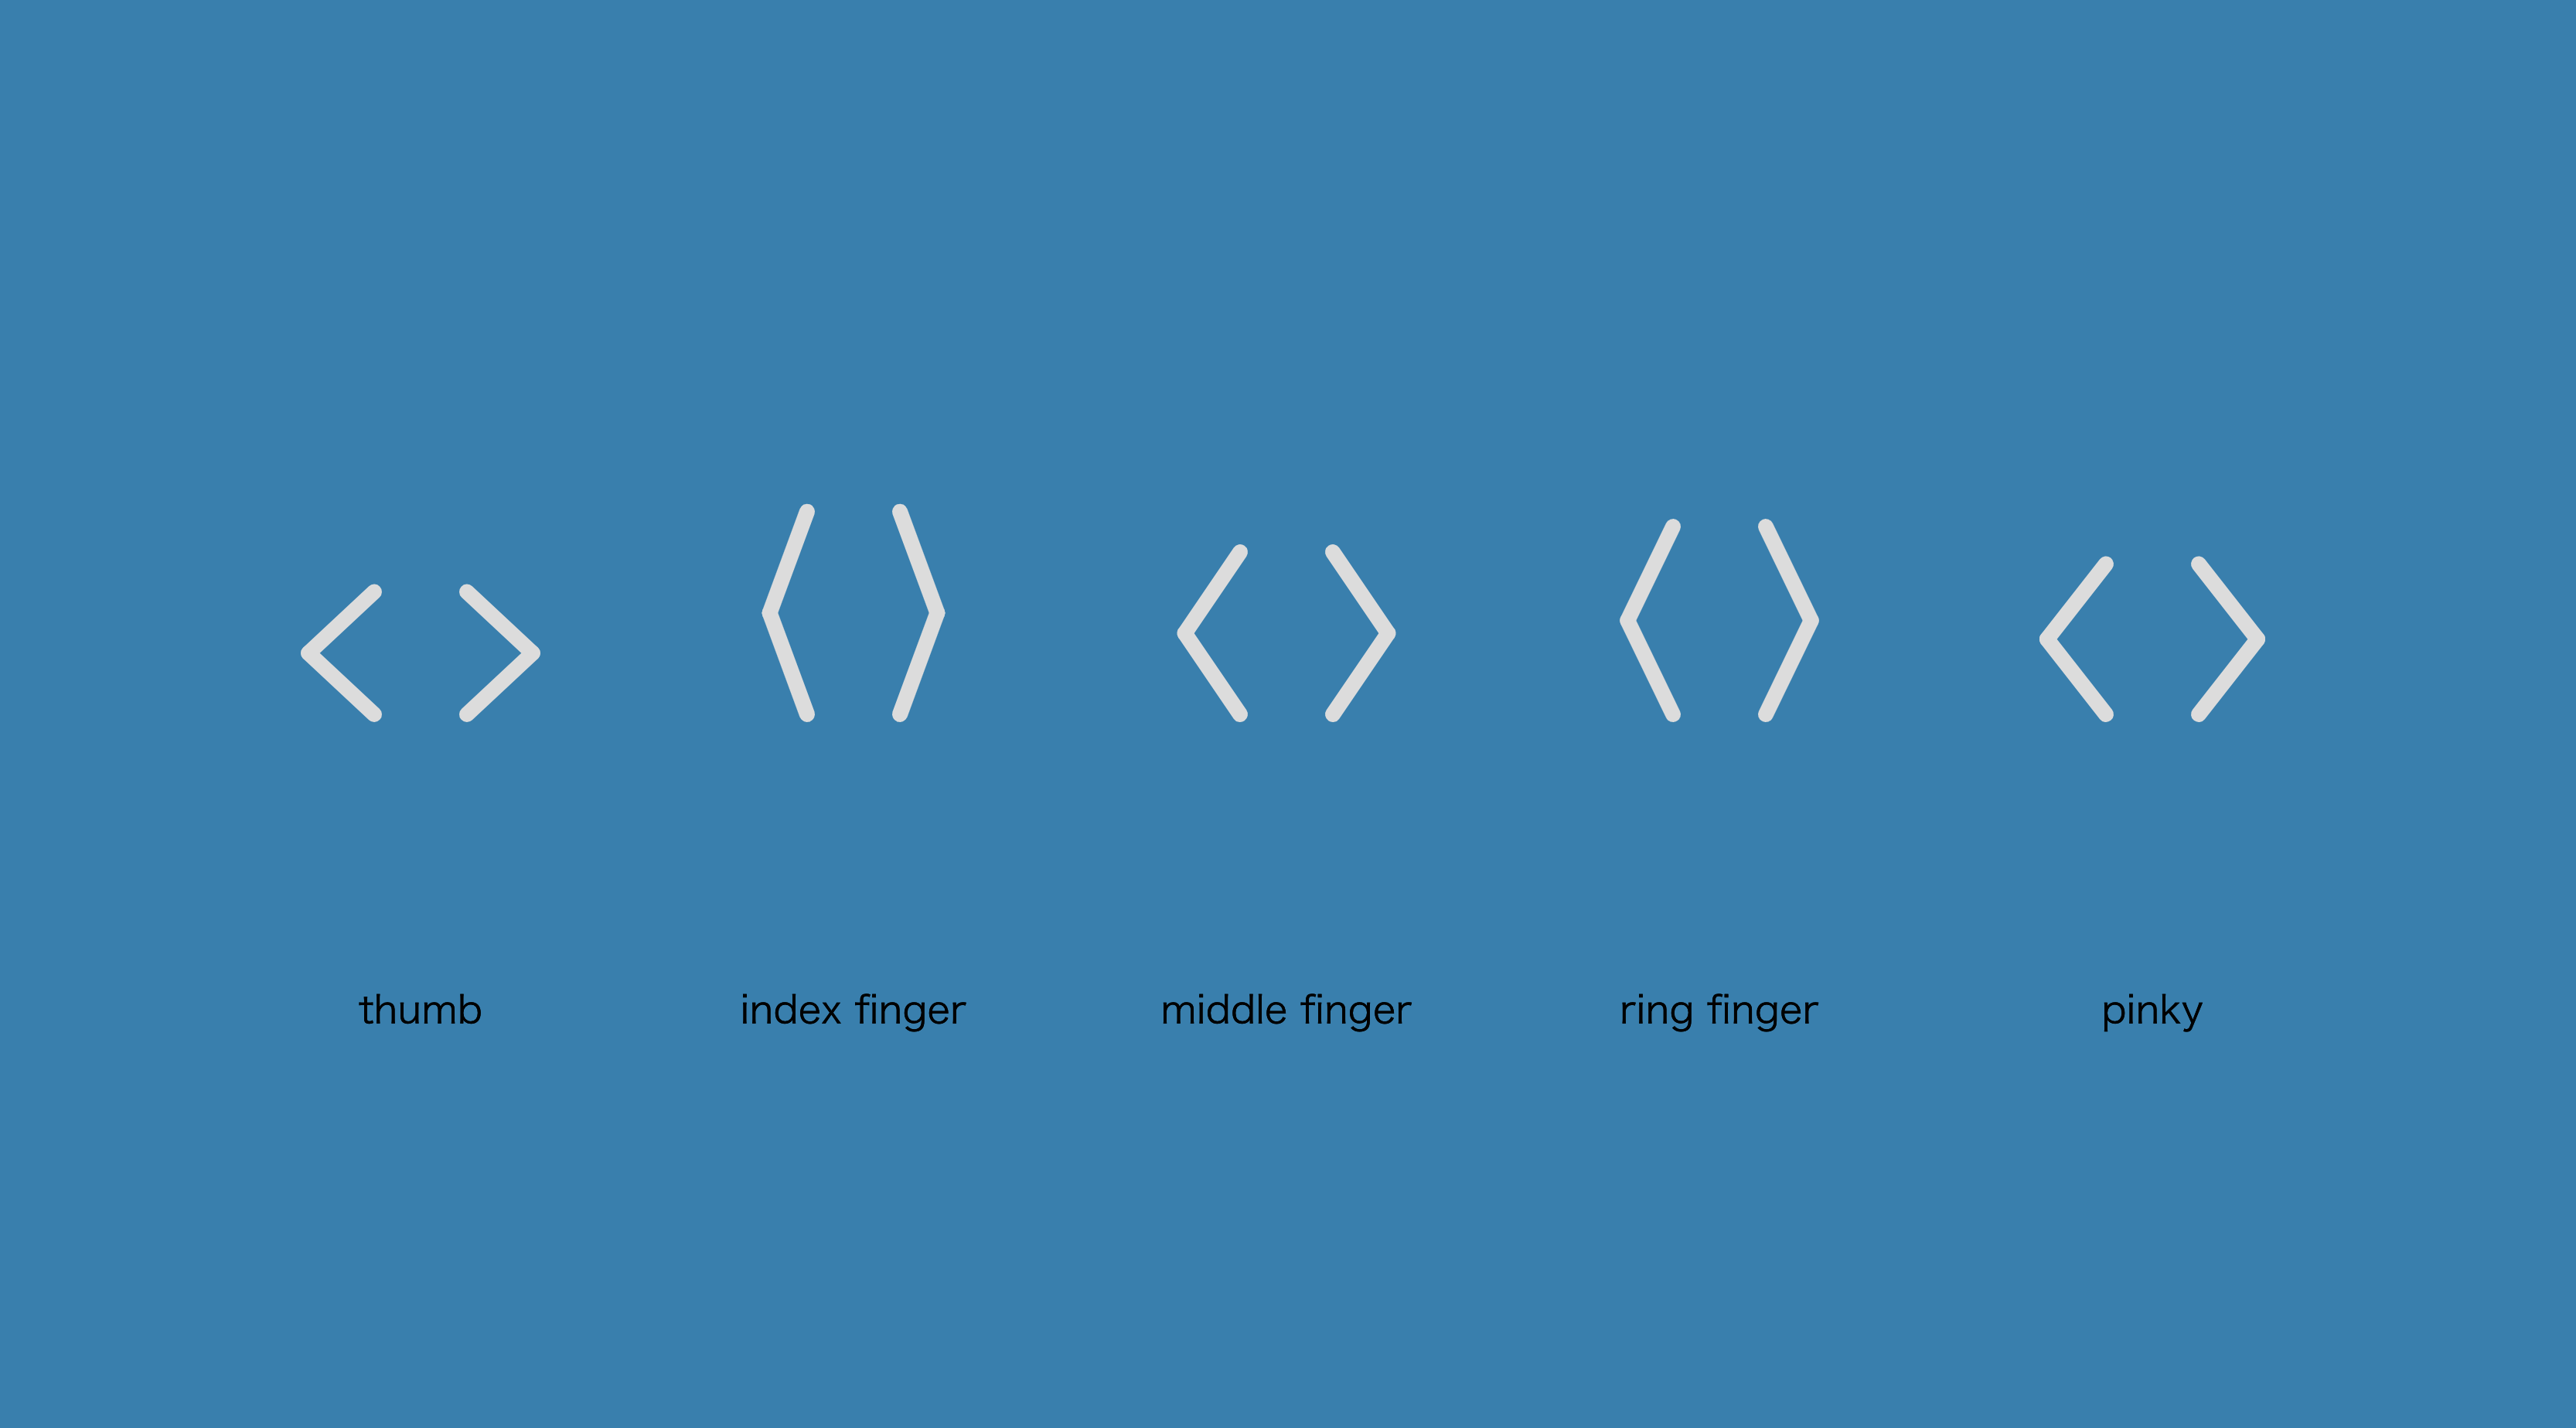
\includegraphics[width=15cm]{img/kunoji_2022.png}
  \caption{「くの字」が並んだパターン(2022年)}
  \label{fig:exhibit_2022_kunoji}
\end{figure}

\begin{figure}[htbp]
  \begin{minipage}[b]{0.5\linewidth}
    \centering
    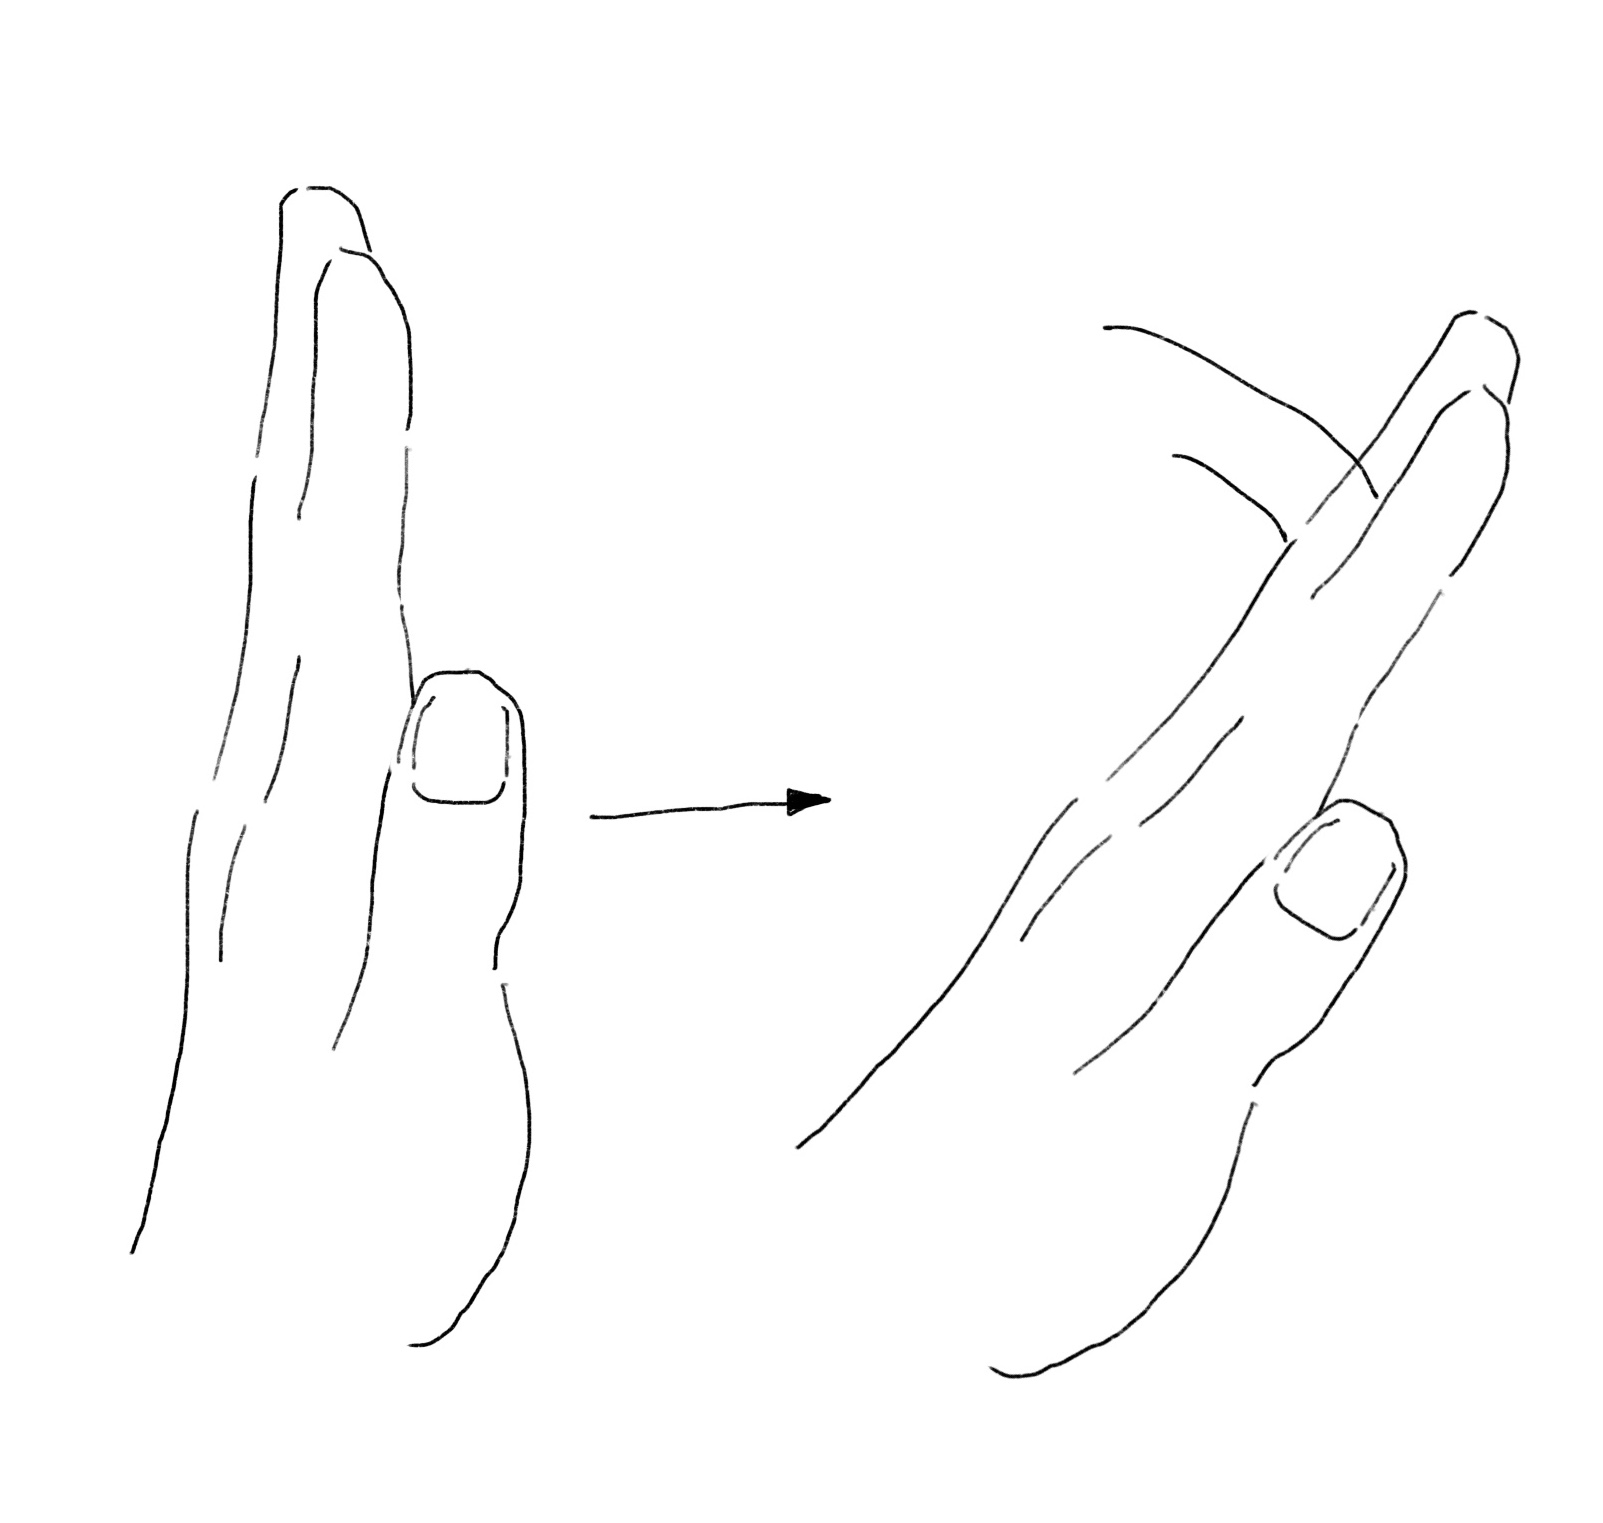
\includegraphics[keepaspectratio, width=7cm]{img/movement0.jpg}
    \caption{手首を軸に動かす体験者の動き}
    \label{fig:movement_0}
  \end{minipage}
  \begin{minipage}[b]{0.5\linewidth}
    \centering
    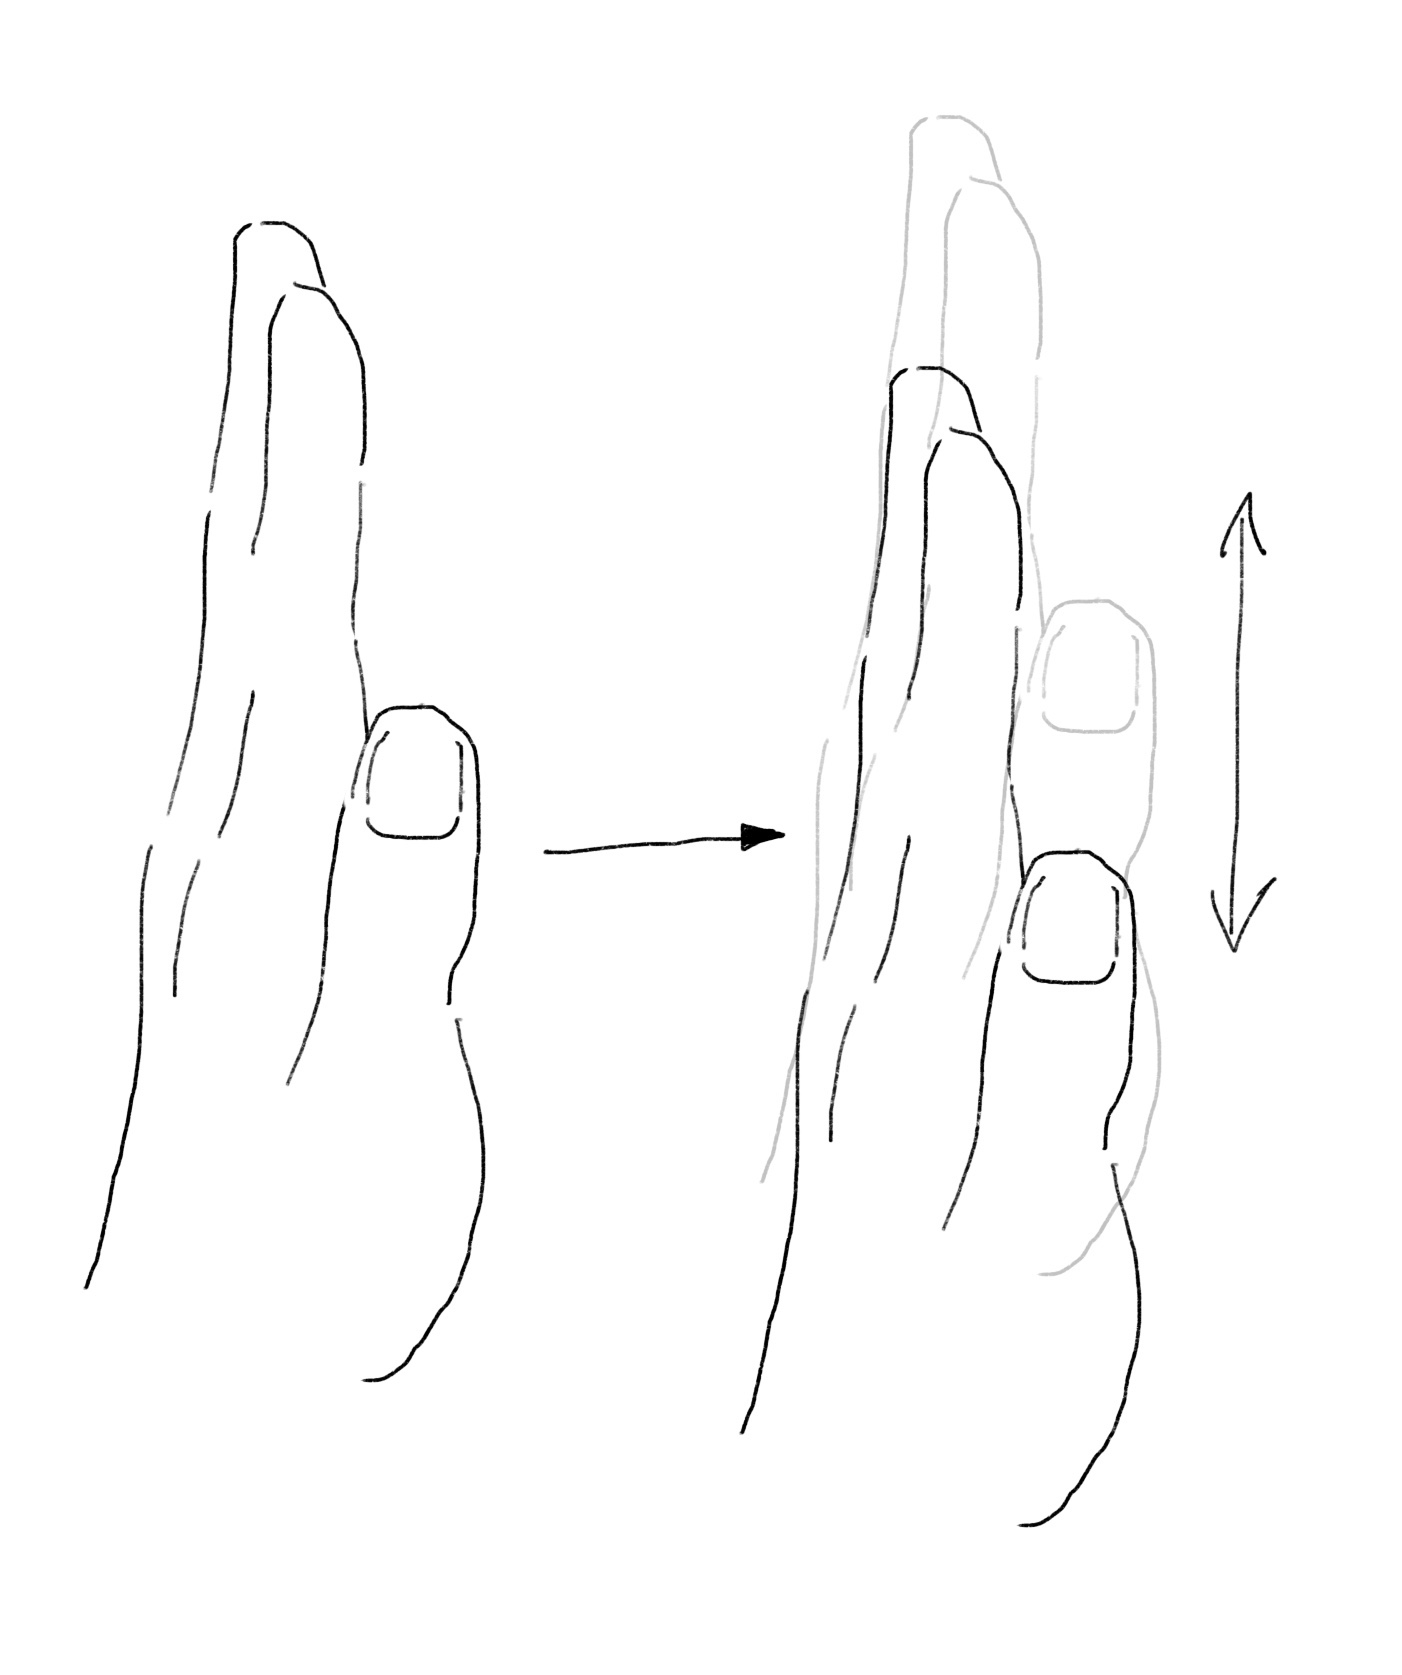
\includegraphics[keepaspectratio, width=7cm]{img/movement1.jpg}
    \caption{トラッキングのズレの挙動で動かす体験者の動き}
    \label{fig:movement_1}
  \end{minipage}
\end{figure}

このように解釈に幅があったことは、2つのことを示唆する。一つは、この形状自体にどのように動かせば良いのかを示唆する記号やアフォーダンスが存在していなかったことである。また、そのために体験者は「動かす」ことを通して理解していたということである。ここに、こうした解釈の余地が生まれ、「唯一性」のあるインタラクションが生じていたことに魅力を感じた。

またこの作品について、10分以上興味を持って体験する人が複数名いた点にも注目した。手指を変換しただけのこの表現に、惹きつけるものがあるのは何か。筆者はここで、「動かすこと自体の快体験」があるのではないかと考えた。対極にあるのは、「動かした反応から得られる快体験」である。そうではなく、指一本一本の細やかな動きに連動して、緻密に動かしている感覚が、この体験の魅力的な部分になるのではないかと考えた。

ここまで見てきたように、この表現には「動かすことで解釈が生まれる」からこその「唯一性」のあるインタラクション、そして「動かすこと自体の快体験」があると考えた。これは、先に提起した「他者に帰属する私たち」のような関係性を喚起する上で、重要なエッセンスになりうる。そのため、本研究ではこれらの特性をもつ「手指の変換表現」から「人馬一体感」について探求し、そのデザインを目指した。

\section{本研究の目的}

本研究の目的は、人と道具や機械における「人馬一体」のような一体感をデザインするための指針や具現化するための方法を明らかにすることである。

本研究では、手指の変換表現からアプローチした。探索的におこなったプロトタイピングの中から、その生起に関わると考えられる要素について検討した。そして、その要素から構成された修士作品《Grasp(er)》を制作した。随所に「人馬一体感」が生起することをねらいとして構成されたこの作品の体験を、「``一体化''としてのembodiment」から人と対象との関係を分類したとみられるコンピュータ工学者Sydney Felsの提唱する概念を用いて捉えることで、それが何を達成するデザインであったのかについての仮説を立てる。その検証のため、本作について4名の作品体験を振り返ることから何が達成できていたのか、そしてその上でこの一体感をデザインする上で重要となる指標が何かについて論じる。

\section{本論文の構成}
本章では、研究背景と概要を示した。また、本研究が「手指とは異なる形状への変換」の観点からこのテーマに取り組むことの動機として、過去の習作《Digitize》を通した気づきについて説明した。

第\ref{related_works}章では、「embodiment」に関する先行研究について、``身体化''を扱う側面と``一体化''を扱う側面があることを指摘し、その中での本研究の位置付けと貢献を示す。

第\ref{prototyping}章では、手指の変換表現についての探索と、「人馬一体感」の生起に向けた意識的な試行が生じる体験として作品を構成するにあたっての取捨選択のプロセスを説明し、最終的な作品における構成の根拠を示す。

第\ref{about_grasper}章では、作品概要と、作品におけるねらいをSydney Felsが定義したembodimentの分類に基づいて示す。

第\ref{validation}章では、前章に示したねらいのもと構成された《Grasp(er)》が、実際どのように体験されたのかを調査するための方法と、その結果を示す。

第\ref{考察}章では、行った調査の結果を本作品のねらいと照らし合わせた上で、この作品がどのように体験されていたのかについて分析し、Felsの分類を用いる限りでは捉えきれなかった作品と参加者の関係性について指摘する。

第\ref{matome}章では、これまでの議論をまとめ、本研究の目的に照らし合わせた上で、作品制作と体験の分析を通して明らかとなったことについて述べる。